\chapter{Structural Causal Model}
\section{Structural Causal Models}
Graphical causal models such as causal bayesian network give us powerful ways to
encode statistical and causal assumptions, but we have yet to explain exactly
what an \textit{intervention} is or exactly what a \textit{causal mechanism} is.

Moving from causal Bayesian networks to \textbf{full Structural causal models}
will give us this additional clarity along with the power to compute \textbf{counterfactuals}.

We need a way to specify the following concept:
\begin{center}
    $A$ causes $B$
\end{center}
this means that changing $A$ changing also $B$ but changing $B$ doesn't mean changing $A$.

We use the notation $B := f(A)$, which means that we assign to $B$ the value of
$f(A)$. This symbol ($:=$) denotes an \textbf{asymmetric assignment} and differs
from the symmetric equality symbol ($=$).

\begin{note}
    Using $B := f(A)$ we are using a \textbf{causal model}, while $B = f(A)$ we
    are using a \textbf{statistical model}
\end{note}

This operator ($:=$) is deterministic. Ideally, we'd like to allow it to be
probabilistic, which allows room for some unknown causes ($U$) of $B$ that factor
into this mapping. Then, we write the \textbf{structural equation} as:
\begin{equation*}
    B := f(A, U)
\end{equation*}
This means that the function $f$ is deterministic (is a stochastic mapping)
applied on $A$ that we know with some noise $U$ that models the unknown causes.
An example of this is reported in Figure~\ref{fig:unknown_graphs}.

\begin{figure}[!ht]
    \centering
    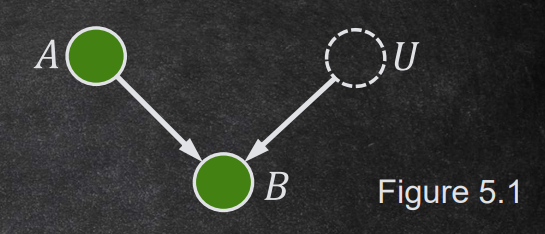
\includegraphics[width=0.5\textwidth]{img/structural_causal_model/unknown_graphs.png}
    \caption{Graphical representation of the structural equation}
    \label{fig:unknown_graphs}
\end{figure}

When $f$ is not specified we are in the \textbf{nonparametric regime} because we
aren't making any assumptions about parametric form. However, \textit{structural
    equations} can represent any stochastic mapping, so generalize the
\textit{probabilistic factor}:
\begin{equation*}
    P(X_i | pa(X_i))
\end{equation*}

Therefore, all the results that we've seen such as the truncated factorization
and the backdoor adjustment still hold when we introduce structural equations.

We have now come to the more precise definitions of what a cause is and what a
causal mechanism is.

\begin{definition}[\textbf{Causal Mechanism}]
    A causal mechanism that generates a variable is the structural equation
    that corresponds to that variable.
\end{definition}
\begin{note}
    Cause is more general than directed cause.
\end{note}
From the initial model $B := f(A,U)$ the $A, U$ are directed cause for $B$.

In general, a model can consist of more than one structural equation, for example:
\begin{equation}
    M : \,\, \begin{array}{l}
        B := f_B(A, U_B) \\ C := f_C(A, B, U_c) \\ D := f_D(A, C, U_D)
    \end{array}
\end{equation}
Starting from this model we can build the associated causal graph, where we draw
an edge from every variable on the right-hand side to the variable on the left-hand side.
The associate causal graph is reported in Figure~\ref{fig:associate_graph}.
\begin{figure}[!ht]
    \centering
    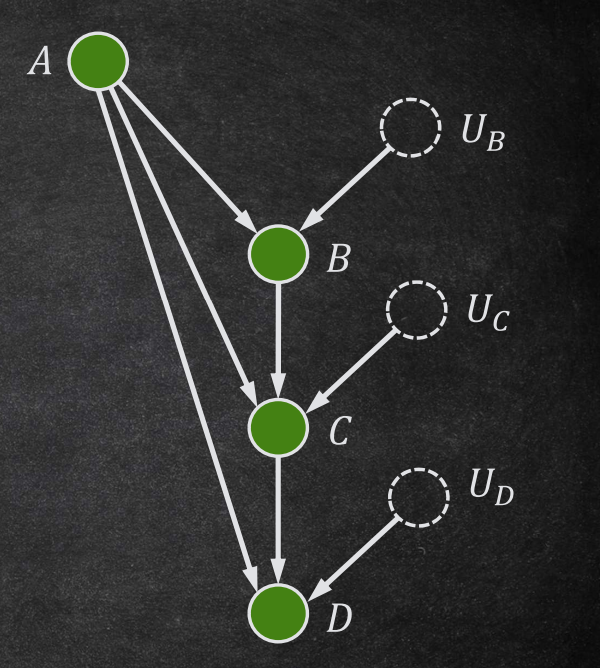
\includegraphics[width=0.35\textwidth]{img/structural_causal_model/graph_associate_structural_equation.png}
    \caption{Associate causal graph}
    \label{fig:associate_graph}
\end{figure}

Based on the previous example, we can distinguish $A, U_B, U_C, U_D$ as \textbf{
    exogenous variables}, i.e., they can not be descendant of any other variables,
and in particular, they can not be descendant of an endogenous variable; they have
no ancestors and are represented as root nodes in graphs.

\begin{definition}[\textbf{Exogenous Variables}]
    The exogenous variables are the variables for which we don't have a structural
    equation that explains their behavior, so they are root node in the graph.
\end{definition}

They are external to the model; we chose, for whatever reason, not to explain how
they are caused (we don't care about cause of cause).

While, $B, C, D$ are \textbf{endogenous variables}, i.e., the variables that we
write structural equations for, i.e., the variables whose causal mechanisms we
are modeling.

\begin{definition}[\textbf{Endogenous Variables}]
    The endogenous variables are the variables for which we have a structural
    equations that define their behavior, so they have parents in the graph.
\end{definition}

If we know the value of every \textbf{exogenous variable}, then using the functions
of the structural equations, we can determine with perfect certainty the value
of every \textbf{endogenous variable}.

\begin{definition}[\textbf{Structural Causal Model}]
    A \textbf{structural causal model} (SCM) is a tuple $M = \langle U, V, F \rangle$
    of the following sets:
    \begin{itemize}
        \item $U$ is a set of exogenous variables.
        \item $V$ is a set of endogenous variables.
        \item $F$ is a set of functions, one to generate each endogenous variable
              as a function of other variables.
    \end{itemize}
\end{definition}

Every structural causal model implies an associated \textbf{causal graph}: for each
structural equation, draw an edge from every variable on the right-hand side to the
variable on the left-hand side.

If we have a causal graph contains no cycles (it is a DAG) and the \textbf{noise
    variable} $U$ are:
\begin{itemize}
    \item \textbf{Independent} so the causal model is \textbf{Markovian}
    \item \textbf{Dependent} so the causal model is \textbf{semi-Markovian}
\end{itemize}

\begin{note}
    If there is a \textbf{unobserved confounding} the model is \textbf{semi-Markovian}. And
    the graph of \textbf{non-Markovian} models contains cycles.
\end{note}

\textbf{Interventions} in SCMs consist of replacing the structural equation, i.e.,
if the intervention is $do(X = x)$ then we replace the structural equation associated
with $X$. For example:
\begin{equation}
    M : \begin{array}{l}
        Z := U_Z \\ X := f_X(Z, U_X) \\ Y:= f_Y(X, Z, U_Y)
    \end{array}
\end{equation}
The graph associated is Markovian. If we do the following intervention as $do(X = x)$
so the structural equation will be:
\begin{equation}
    M_X : \begin{array}{l}
        Z := U_Z \\ X := x \\ Y:= f_Y(X, Z, U_Y)
    \end{array}
\end{equation}
and the graph will be modified removing the edge between $U_X$ and $X$. The resulting
graph is reported in Figure~\ref{fig:intervention_graph}.
\begin{figure}[!ht]
    \centering
    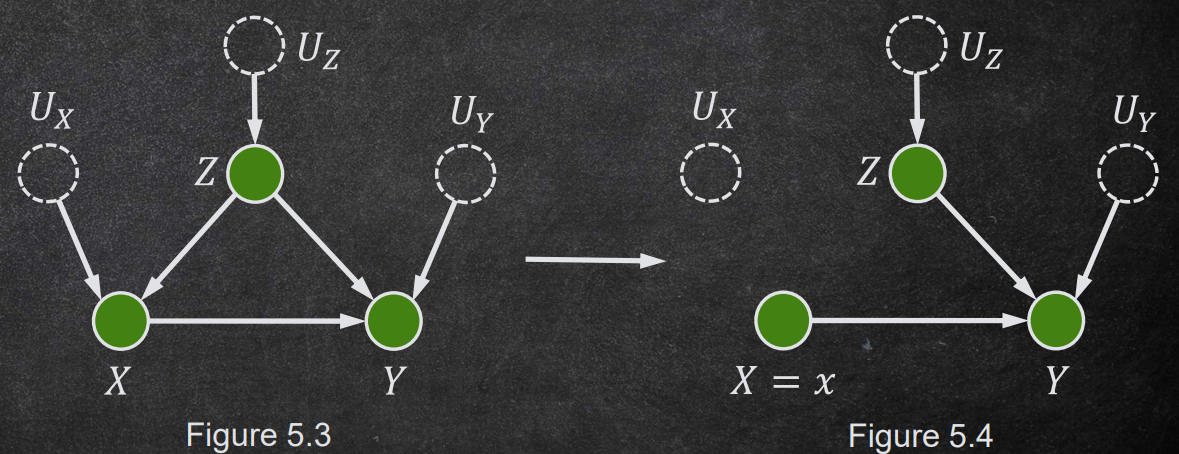
\includegraphics[width=0.5\textwidth]{img/structural_causal_model/intervention_on_structural_eq.png}
    \caption{Intervention on structural equation}
    \label{fig:intervention_graph}
\end{figure}

Only changes the equation for $X$ and no other variables is a consequence of the
\textbf{modularity assumption}; these causal mechanisms are modular.

\begin{definition}[\textbf{Modularity assumption for SCM}]
    Consider an SCM $M = \langle U, V, F \rangle$ and an interventional SCM
    $M_x =\langle U, V, F_x \rangle$, that we get by performing the intervention
    $do(X = x)$.

    The modularity assumption states that $M$ and $M_x$ share all of their
    structural equations except the structural equation for $X$, which is
    $X := x$ in $M_x$.
\end{definition}
For the modularity the intervention $do(X = x)$ is localized to $X$.

We can write unit level potential outcome as:
\begin{itemize}
    \item $Y_x (u)$ potential outcome that unit $u$ would observe if taking treatment
          $X = x$, given that the SCM is $M$.
    \item $Y_{M_x}(u)$ potential outcome that unit $u$ would observe if taking
          treatment $X = x$, given that the SCM is $M_x$ (in the manipulated model).
\end{itemize}

The \textbf{law of counterfactuals} gives us information about counterfactuals:
\begin{equation}
    Y_x(u) = Y_{M_x}(u)
\end{equation}

Given an SCM with enough details about it specified, we can actually compute
counterfactuals. This is extremely important because it is exactly what the
fundamental problem of causal inference told us we cannot do.

Not only did we specify that the adjustment set blocks all backdoor paths from
$X$ to $Y$, but we also specified that does not contain any descendants of $X$,
otherwise we have a selection bias effect.

There are two categories of things that could go wrong if we condition on descendants
of $X$:
\begin{enumerate}
    \item We block the flow of causation from $X$ to $Y$;
    \item We induce non-causal association between $X$ and $Y$, we generate a
          spurious path not existed before.
\end{enumerate}

In the first case, if we have a chain between $X$ and $Y$ and we have at least a
node $L$ that is a \textbf{mediator} of the causal effect of $X$ on $Y$. So when
we observe $L$ we measure a $0$ causal effect between $X$ and $Y$ because it's
blocked by the observation on the mediator.

If we have a mediator with an observation and direct link from $X$ to $Y$ so we
can measure the direct cause effect of $X$ on $Y$ but not the un-direct.

In the second case, if we have a direct link between $X$ and $Y$ and a collider
on $L$ that is a descendant of $X$ and $Y$, if we condition on a descendant of $L$
that isn't a mediator, it could unblock a path from $X$ to $Y$ that was blocked
by a collider, so we are introducing a \textbf{collider bias}. The same holds true
for any descendant of $L$. So we should only control the counterfactuals.

It is worthwhile to notice that we actually can condition on some descendants of
$X$ without inducing non-causal associations between $X$ and $Y$. Conditioning
on descendants of $X$ that aren't on any causal paths from $X$ and $Y$ won't
induce bias.

Even outside of graphical causal models, this rule is often applied; it is usually described
as not conditioning on any \textbf{post treatment variables}.

Unfortunately, even if we only condition on \textbf{pre-treatment covariates}, we
can still induce \textbf{collider bias} if we condition on the collider. Doing
this opens up a backdoor path, along which non-causal association can flow. This
is known as $M$-Bias due to the $M$-Shape that this non-causal association flows
along when the graph is drawn with children below their parents.

\section{Application of Backdoor Adjustment}
In this section we will show how to derive the \textbf{associational} quantity
$\mathbb{E}[Y|X = x]$ (it is the observational value obtained without intervention),
that will be compared to the \textbf{causal} quantity $\mathbb{E}[Y|do(x)]$. There
are situations where the causal quantity is the same to the associational.

If the treatment were binary, then we would just look at the difference between
the quantities with the respected value. However, if we consider \textbf{linear
    generative process}, thus quantities are:
\begin{equation}
    \frac{\partial\mathbb{E}[Y |x]}{\partial x } \, \land \, \frac{\partial\mathbb{E}[Y |do(x)]}{\partial x}
\end{equation}
this formulation give us all the information about the treatment effect, regardless
of if treatment is continuous, binary, or multi-valued.

\begin{note}
    In this section we will assume \textbf{infinite} data so we can work with expectations.
    It's a strong assumption but helps in explain the situation.
\end{note}

For the rest of this section we will consider the example given in Figure~\ref{fig:example}.
This can also be represented as follows:
\begin{equation}
    \begin{array}{l}
        X := \alpha_1 Z \\ Y := \beta X + \alpha_2 Z
    \end{array}
\end{equation}
where $\beta$ is the causal effect of $X$ on $Y$ and $\alpha_1, \alpha_2, \beta \in \mathbb{R}$.
\begin{figure}[!ht]
    \centering
    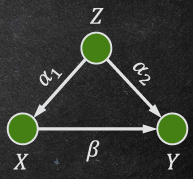
\includegraphics[width=0.2\textwidth]{img/structural_causal_model/example.png}
    \caption{Basic example}
    \label{fig:example}
\end{figure}

Let's now prove that $ beta$ is the causal effect of $X$ on $Y$. Given the ordered
pair $(X, Y)$ and the set $S = \{Z\}$ which represents the \textbf{sufficient
    adjustment set} we have the following:
\begin{equation}
    \begin{array}{ll}
        \mathbb{E}[Y | do(x)] = \mathbb{E}_Z[\mathbb{E}[Y | X = x, Z]] & = \mathbb{E}_Z[\mathbb{E}[\beta X + \alpha_2 Z | X = x, Z]] \\
                                                                       & = \mathbb{E}_Z[\mathbb{E}[\beta x + \alpha_2 Z]]            \\
                                                                       & = \mathbb{E}_Z[\beta x + \alpha_2 Z]                        \\
                                                                       & = \beta x + \alpha_2\mathbb{E}[Z]
    \end{array}
\end{equation}
then, we have the following:
\begin{equation}
    \frac{\partial \mathbb{E}[Y |do(x)]}{\partial x} = \frac{\partial [\beta x + \alpha_2\mathbb{E}[Z]]}{\partial x} = \beta
\end{equation}

While, when we are talking about \textbf{associational effect} from $X$ to $Y$ we have:
\begin{equation}
    \begin{array}{ll}
        \mathbb{E}[Y | x] = \mathbb{E}[Y | X = x] & = \mathbb{E}[\beta X + \alpha_2 Z | X = x] \\
                                                  & = \beta x + \mathbb{E}[\alpha_2 Z |X = x]  \\
                                                  & = \beta x + \alpha_2 \mathbb{E}[Z |X = x]  \\
                                                  & = \beta x + \frac{\alpha_2}{\alpha_1} x
    \end{array}
\end{equation}
then, we have the following:
\begin{equation}
    \frac{\partial \mathbb{E}[Y |x]}{\partial x} = \frac{\partial[\beta x + \alpha_2 \mathbb{E}[Z |X = x]]}{\partial x} = \beta + \frac{\alpha_2}{\alpha_1}
\end{equation}
Therefore, it is clear that \textbf{associational effect} of  $X$ on $Y$ is
different from the \textbf{causal effect} of $X$ on $Y$.

In the potential outcomes framework, it is common to only condition on pre-treatment
covariates. This would prevent a practitioner who adheres to this rule from
conditioning on the collider. However, there is no reason that there can't be
pre-treatment colliders that induce $M$ bias.

Given, the \textbf{modularity assumption} and \textbf{markov assumption} and
\textbf{positivity}, if the backdoor criterion is satisfied in our assumed causal
graph, then we achieve \textbf{identification}.

\begin{note}
    Note that although the a backdoor criterion is a sufficient condition for
    identification, it is not a necessary condition.
\end{note}
\begin{note}
    No interference assumption in commonly implicit in causal graph because the $Y$
    usually only has a single node $X$ for treatment as a parent. In other way
    consistency follows from the axioms of SCMs. Contrary the positivity is still
    important assumption that we must make.
\end{note}

